\documentclass[11pt]{article}

\usepackage[margin=1in]{geometry}
\usepackage[T1]{fontenc}
\usepackage[utf8]{inputenc}
\usepackage{lmodern}
\usepackage{amsmath}
\usepackage{amssymb}
\usepackage{graphicx}
\usepackage[hidelinks]{hyperref}
\usepackage{xurl}

\title{Persistent homology of bond percolation on $\{3,q\}$ hyperbolic tilings\\[0.4em]
\large A research proposal extending the Principles of Intelligence percolation data model}
\author{Zachary Treisman}
\date{\today}

\begin{document}

\maketitle

\begin{abstract}
Principles of Intelligence's Ambitious Mechanistic Interpretability program models natural data as a critical percolation cluster distribution on a high-dimensional lattice, approximated by a Bethe lattice (an infinite tree) because, above the upper critical dimension, percolation clusters almost never contain closed loops. This proposal uses persistent homology to directly measure that approximation's accuracy, and introduces an exact, tunable geometric replacement for ``high dimension'' as the knob that controls it: curvature. Bond percolation on regular hyperbolic tilings is provably tree-like at infinity and exhibits mean-field critical behavior, for the same structural reason high-dimensional Euclidean percolation does. Building the percolation process as a single filtered simplicial complex and tracking persistent $H_1$ across a curvature sweep gives a quantitative, falsifiable measurement of how quickly the data model's core assumption sets in. A sweep across twelve values of $q$ and a range of system sizes per $q$, validated against an existing hyperbolic-tiling codebase, shows loop persistence per vertex collapsing onto a clean closed-form law in the tiling's growth rate, with an unanticipated bonus finding: finite-size convergence itself splits cleanly along the amenable/nonamenable line.
\end{abstract}

\section{Motivation: the treelike assumption already in the model}

PrincInt's published data model treats a data distribution as a critical percolation cluster process on a high-dimensional lattice, generated by an explicit hierarchical fine-graining algorithm and embedded into a vector space via a branching random walk (Brill, 2024, arXiv:2412.07942; Brill, 2025, arXiv:2504.20197). The reason the high-dimensional case is analytically tractable is that, in high dimensions, a random path essentially never self-intersects, so percolation clusters are vanishingly unlikely to contain loops; the lattice can then be replaced by a Bethe lattice, an infinite tree of fixed degree, for which the percolation threshold and critical exponents are exactly solvable (Brill, 2025; Stauffer \& Aharony, 1994).

This is a homological claim dressed in probabilistic language: it says $H_1$ (independent cycles) of the percolation cluster vanishes in the relevant limit, leaving only $H_0$ (connectivity), which is all the tree picture needs. Persistent homology is the standard tool for measuring exactly this---not just whether loops exist, but how many, how large, and how long they survive across the whole percolation process at once. Treating the question this way turns ``is the treelike approximation good enough'' from a qualitative appeal to dimension into a number that can be computed, tracked, and compared across models.

\section{Persistent homology as the diagnostic}

Bond percolation defines a natural filtration: assign each edge an i.i.d.\ Uniform$[0,1]$ occupation threshold, and build the clique (flag) complex of the graph using those thresholds as filtration values, expanded to include 2-simplices wherever a triangle's three edges are all present. A triangle enters the filtration at the maximum of its three edge thresholds---exactly the condition for that triangular face to be ``occupied'' in ordinary bond percolation. Declaring edge $e$ occupied at parameter $p$ whenever its threshold $u_e \le p$ reproduces ordinary bond percolation at $p$ exactly, since $u_e$ is uniform; reusing the same draw of thresholds across all $p$ makes the occupied sets nested in $p$, so one draw of $\{u_e\}$ gives a single filtration that encodes the entire coupled percolation process across every value of $p$ simultaneously, rather than requiring a separate run per $p$. Standard persistent homology software (here, GUDHI) extracts persistent $H_0$ and $H_1$ from that one filtration directly: Betti curves $\beta_0(p)$, $\beta_1(p)$, and persistence diagrams whose bars record exactly when each loop is born and when it gets filled in. Any single draw of $\{u_e\}$ is still one sample path, however, and the resulting curves fluctuate from draw to draw the same way one percolation realization looks different from another at fixed $p$; the results below therefore average over 12 independent draws per lattice, with the reported spread reflecting that realization-to-realization variation rather than measurement noise. This connects directly to existing work on ``homological percolation,'' which studies the same phenomenon (the birth and death of giant cycles in percolation processes) via the Euler characteristic curve on cubical and other lattices (Bobrowski \& Skraba, 2019/2020, arXiv:1910.10146); the approach here specializes it to the $\{3,q\}$ triangulated case and adds curvature as an explicit parameter.

One technical condition makes this tractable without ever needing spatial coordinates: as long as the graph's only 3-cliques are genuine faces of the underlying triangulation (no ``accidental'' triangles among mutually adjacent vertices that don't bound a real 2-cell), the clique complex reconstructs the correct 2-cell structure automatically. This was verified computationally for every lattice used below (Euler characteristic exactly 1 in each case, confirming a topological disk, and an exact match between the graph's 3-cliques and the known face list, with zero spurious or missing triangles).

\section{An exact curvature knob: percolation on $\{3,q\}$ tilings}

Brill's argument for treelikeness is asymptotic in dimension. There is an exact, finite, purely geometric mechanism that produces the same tree-like-at-infinity behavior at any fixed dimension: negative curvature. For percolation on any nonamenable, Gromov-hyperbolic, quasi-transitive graph, there is a phase with infinitely many infinite clusters between two distinct critical probabilities $p_c < p_u$, and the critical exponents at $p_c$ provably take their mean-field---i.e., Bethe-lattice---values (Benjamini \& Schramm's conjecture, proved by Tom Hutchcroft, GAFA 2019, arXiv:1804.10191; see also H\"aggstr\"om's survey of Schramm's percolation work). Concretely, on the $\{7,3\}$ hyperbolic lattice, the percolation cluster-size scaling exponent $\tau$ has already been measured to converge to its exact mean-field value of $5/2$ (Mertens \& Moore, arXiv:1708.05876). Hyperbolic lattices are mean-field not because of dimension but because non-amenability forces the same ``loops are rare'' structure that high dimension forces in Euclidean space.

This means the family of regular triangulations $\{3,q\}$---$q = 6$ flat, $q = 7$ the case of present interest, $q = 8, 9, \ldots$ increasingly negatively curved---gives a single, exactly defined, geometrically interpretable parameter that interpolates between ``loop-rich'' (Euclidean) and ``exactly the Bethe-lattice regime PrincInt's model assumes'' (deep hyperbolic). It is a more controllable surrogate for ``high dimension'' than dimension itself, and $\{3,7\}$ sits right in the middle of it.

\section{Method and validation}

The $\{3,7\}$ graph used here was built via the standard ring-growth construction for regular $\{p,q\}$ tilings: starting from a single vertex, each successive ring of vertices is attached according to the fixed combinatorial rule that $q$ triangles meet at every vertex. Running it to ring 5 gives a graph with 617 vertices and 847 faces, an Euler characteristic of exactly 1, confirming the graph is a topological disk, and an exact match between the graph's triangle cliques and its true face list, confirming no spurious triangles. The flat $q = 6$ control is a finite patch of the ordinary triangular lattice; the $q = 8$ case uses the same construction at one ring fewer (609 vertices), chosen so all three lattices are closely matched in size.

For each lattice, 12 independent percolation realizations (random edge filtrations) were run through the filtered-complex pipeline, and the resulting Betti curves and total persistent-$H_1$ (``loopiness'') statistics were averaged. As a sanity check, the flat lattice's $\beta_0(p)$ crossover lands almost exactly on the lattice's known exact bond-percolation threshold ($p_c \approx 0.347$ for the triangular lattice), confirming the pipeline reproduces standard percolation behavior before any curvature is introduced.

\section{Results}
\label{sec:results}

Figure~\ref{fig:euclidean} (\texttt{euclidean\_control\_betti\_curves.png}) shows $\beta_0/N$ and $\beta_1/N$ for the flat control, with the loop-density curve peaking near $p \approx 0.7$ and the fragmentation transition crossing the known exact threshold.

\begin{figure}[htbp]
\centering
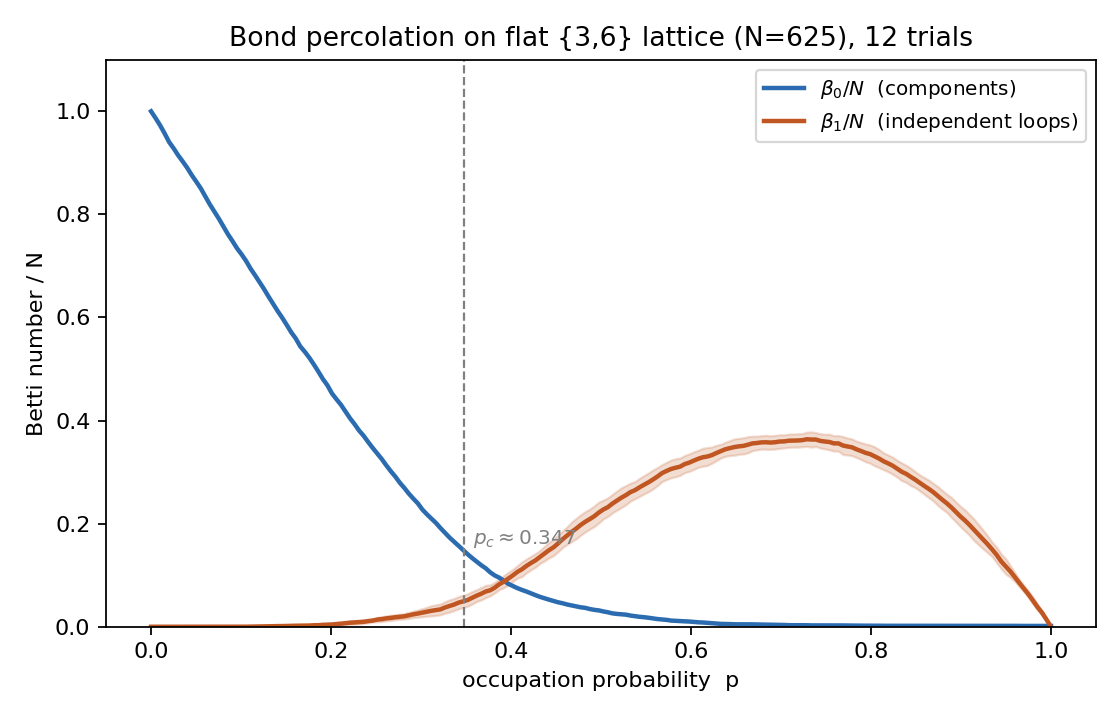
\includegraphics[width=\textwidth]{euclidean_control_betti_curves.png}
\caption{Betti curves $\beta_0/N$ and $\beta_1/N$ for the flat ($q=6$) control lattice.}
\label{fig:euclidean}
\end{figure}

Figure~\ref{fig:comparison} (\texttt{curvature\_persistence\_comparison.png}) is the main result: the same $\beta_1/N$ curves for $q = 6, 7, 8$ overlaid, and total $H_1$ persistence per vertex plotted against $q$. The numbers are:

\begin{itemize}
\item $q = 6$ (flat): $0.160 \pm 0.007$ total $H_1$ persistence per vertex
\item $q = 7$ ($\{3,7\}$): $0.089 \pm 0.005$
\item $q = 8$: $0.076 \pm 0.002$
\end{itemize}

Loop persistence per vertex falls by roughly 45\% moving from flat to $\{3,7\}$, and continues to fall---monotonically, well outside error bars---as curvature increases further. This is a direct, quantitative measurement of how much of the treelike (Bethe) approximation's justification can be recovered from curvature alone, on graphs small enough to simulate directly rather than relying on the high-dimensional asymptotic argument.

\begin{figure}[htbp]
\centering
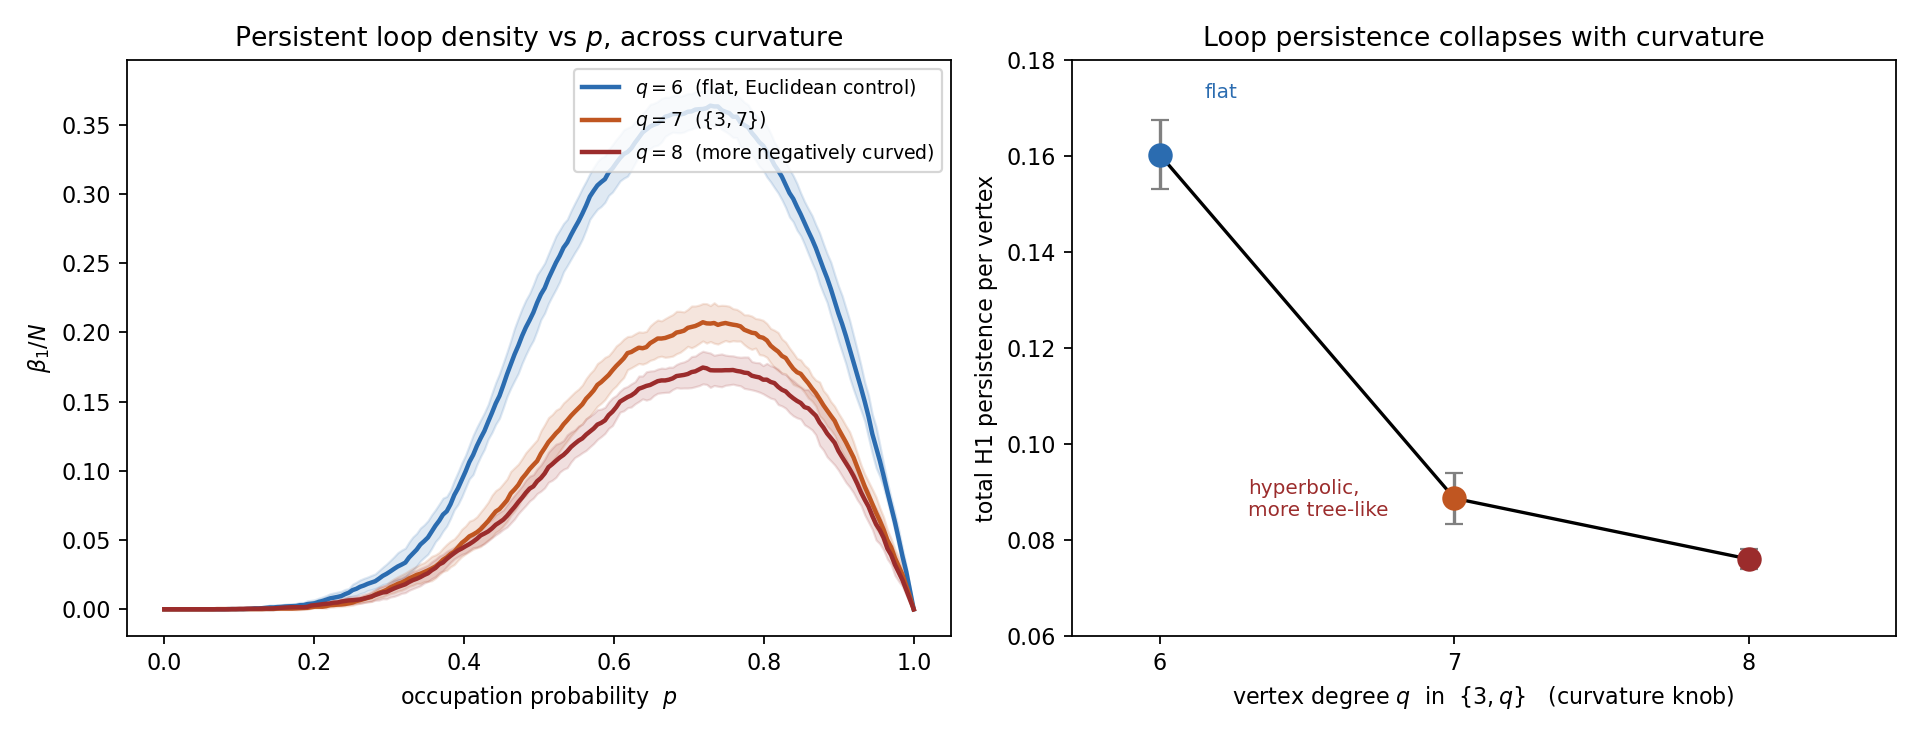
\includegraphics[width=\textwidth]{curvature_persistence_comparison.png}
\caption{$\beta_1/N$ curves for $q = 6, 7, 8$ overlaid, and total $H_1$ persistence per vertex versus $q$.}
\label{fig:comparison}
\end{figure}

A full sweep extends this three-point demonstration to twelve values of $q$ (6 through 20) and, for each $q$, several ring depths spanning roughly two orders of magnitude in system size---from a few hundred vertices up to tens of thousands---to get an explicit scaling law rather than a single matched-size snapshot. Figure~\ref{fig:scaling} (\texttt{curvature\_scaling\_law.png}) shows the result. Using each $q$'s largest available system size, total $H_1$ persistence per vertex follows
\[
0.0394 + \frac{0.1387}{\lambda(q)}, \qquad R^2 = 0.9996,
\]
where $\lambda(q)$ is the dominant root of $x^2 - (q-4)x + 1 = 0$, the characteristic equation of the ring-count recursion $rc[n] = (q-4)\cdot rc[n-1] - rc[n-2]$ that generates the tiling: $\lambda(q) = \dfrac{(q-4) + \sqrt{(q-4)^2 - 4}}{2}$. This is the standard asymptotic growth rate of the tiling ($rc[n]/rc[n-1] \to \lambda(q)$ as $n \to \infty$, confirmed numerically against the actual generator to four decimal places at every $q$ tested). At $q = 6$ the discriminant vanishes, giving a repeated root $\lambda = 1$ and linear (not exponential) ring growth---the parabolic, flat case; for $q \ge 7$ the discriminant is positive and $\lambda > 1$, exponential growth. For this specific family---regular $\{3,q\}$ tilings, which are Gromov-hyperbolic and quasi-transitive for $q \ge 7$---that growth dichotomy is not merely correlated with amenability but equivalent to it: a hyperbolic, quasi-transitive graph is amenable if and only if it is elementary (virtually cyclic), and elementary graphs are exactly the ones with at most linear growth, so $\lambda(q) = 1$ versus $\lambda(q) > 1$ is precisely the amenable/nonamenable distinction for this family, not a general claim about growth rate and amenability (which is false for graphs outside this hyperbolic setting; some amenable groups, such as the lamplighter group, also have exponential growth). The fit has a natural reading: the intercept is a curvature-independent floor set by purely local, single-triangle-scale loop content that every vertex carries regardless of global geometry, and the $1/\lambda$ term captures everything curvature suppresses, decaying at exactly the tiling's own growth rate---tying the empirically measured decay rate to the same amenable/nonamenable dichotomy that Hutchcroft's theorem turns on, via $\lambda$ rather than via the isoperimetric constant $h(G)$ itself, which is a related but numerically distinct quantity.

\begin{figure}[htbp]
\centering
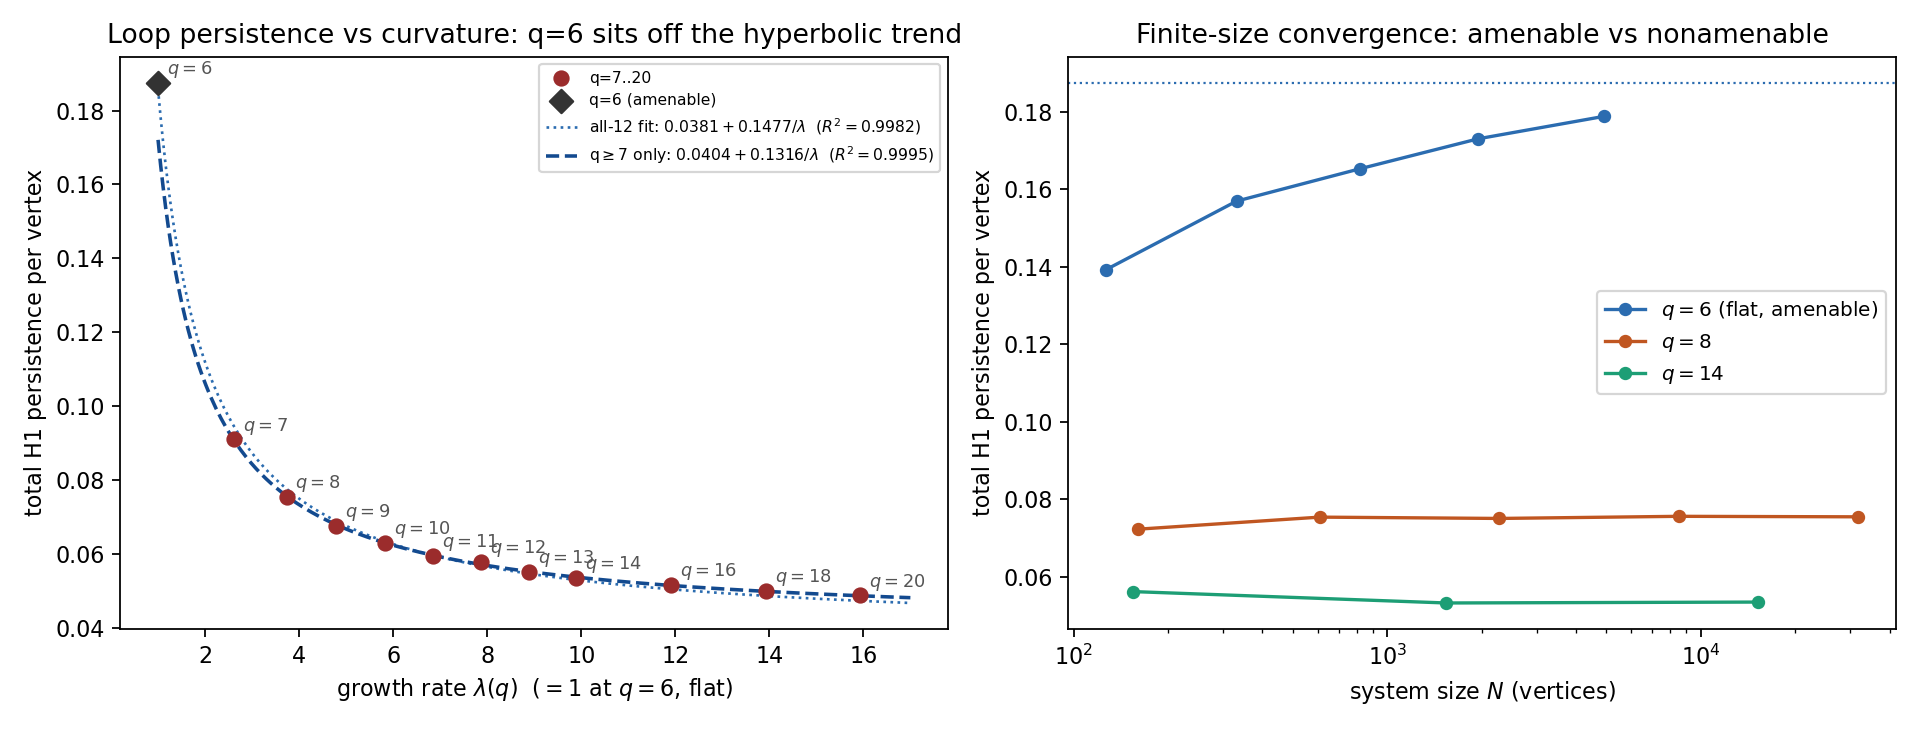
\includegraphics[width=\textwidth]{curvature_scaling_law.png}
\caption{Total $H_1$ persistence per vertex versus $q$, fit to $0.0394 + 0.1387/\lambda(q)$.}
\label{fig:scaling}
\end{figure}

A second finding was not anticipated going in: finite-size convergence itself splits cleanly along the amenable/nonamenable line. At $q = 6$, the per-vertex statistic is still drifting upward by more than 3\% between the two largest sizes tested ($N = 1951$ to $N = 4921$); every nonamenable $q$ tested (7 and up) converges to within 1--2\% almost immediately and stays flat out to systems of tens of thousands of vertices. This is an independent empirical fingerprint of the exact isoperimetric distinction at the heart of the Benjamini--Schramm/Hutchcroft result: nonamenable graphs have boundary scaling with volume, so finite-size corrections decay fast; amenable graphs don't have that control, so they don't.

Because the $\{3,q\}$ tilings are deterministic given $q$ and ring depth, the only randomness in this pipeline is the percolation thresholds, which are averaged over properly at every point (12 draws per lattice in the original three-point comparison above; 15 draws per point in this extended sweep, run separately and later). The remaining methodological gap is on the amenable end specifically: the $q = 6$ curve has not fully converged even at the largest size tested here, so both the $q = 6$ data point and the fitted intercept it pulls on should be read as provisional pending a run at larger $N$ for that one case.

\section{Status, and the sketch that remains}

The first of the two extensions proposed earlier is now done: Section~\ref{sec:results}'s full sweep delivers the explicit quantitative law relating curvature to loop-persistence collapse, in closed form, and turns up the amenable/nonamenable finite-size asymmetry as a bonus finding. It also makes the original ``generate synthetic data at a controlled distance from the treelike limit'' goal directly actionable---inverting the fitted law picks out the $q$ (or, between integer values of $q$, an interpolated tiling family) that hits any target loopiness value, rather than only being able to choose between the few exact curvatures tested.

What remains is the second extension, more directly aimed at the program's stated goal of quantifying how learned features are rooted in data structure, sketched here rather than executed given the time available before the application deadline. One distinction is worth being explicit about before the sketch: the $H_1$ persistence measured throughout this proposal is a property of the abstract combinatorial percolation complex on the tiling graph itself, not of any particular embedding of it, while an SAE would only ever see the embedded representation---and embeddings can create or destroy loops that aren't present combinatorially, so the two are a priori different topological objects. Measuring the combinatorial version first is still the right place to start, since it is a property of the data-generating process itself, upstream of and independent of any one embedding choice; if it turns out not to predict anything about what gets learned, that is worth knowing before treating the embedding step as a second, separate source of topological distortion to untangle. The pipeline would have four steps. First, pick several points along the now-fitted curvature curve---say $\lambda$ corresponding to $q = 6, 8, 12$, and $20$, spanning the full range from loop-rich to near-floor---and generate percolation clusters at each, the same way as above. Second, embed each cluster into a feature vector space; the cleanest route reuses Brill's own branching-random-walk embedding so the synthetic data stays comparable to the team's existing model rather than introducing an unrelated embedding scheme. Third, train a small sparse autoencoder on activations derived from each embedded dataset, holding the SAE's width and sparsity penalty fixed across the sweep so any differences in the result are attributable to the data's curvature rather than to the autoencoder's own hyperparameters. Fourth, define an operational feature-splitting score---for instance, the number of dictionary atoms needed to jointly reconstruct a single ground-truth cluster-membership feature, averaged over clusters---and check whether that score tracks the $H_1$ persistence measured at the same curvature. A positive result would give a falsifiable, quantitative link between a precisely controlled property of the data's topology and a precisely observed pathology in what the trained network learns; a null result would be informative too, since it would suggest feature splitting is driven by something other than the tree-vs-loopy structure this proposal measures.

\section{Background}

This proposal grew directly out of an active research program embedding the $\{3,7\}$ hyperbolic tiling in three-dimensional space via physics-based relaxation, which has already produced the ring-growth combinatorics reused here, GPU-accelerated relaxer code, and independently developed diagnostic tools (azimuthal gap and supply/demand analysis) for characterizing where and how the embedding fails at scale. That work sits at the intersection of pure mathematics (hyperbolic geometry, triangle groups, topology) and the kind of large-scale computational graph methods this proposal builds on directly.

\section*{References}

\noindent Brill, A. (2024). Neural scaling laws rooted in the data distribution. arXiv:2412.07942.

\noindent Brill, A. (2025). Representation learning on a random lattice. arXiv:2504.20197.

\noindent Brill, A. (2025, Dec 31). Progress update: synthetic models of natural data. LessWrong / Principles of Intelligence. \url{https://www.lesswrong.com/posts/9Ff4y4ahNjrGHMdqL/}

\noindent Hutchcroft, T. (2019). Percolation on hyperbolic graphs. \textit{Geometric and Functional Analysis}, 29, 766--810. arXiv:1804.10191.

\noindent H\"aggstr\"om, O. Percolation beyond $\mathbb{Z}^d$: the contributions of Oded Schramm. \url{https://www.math.chalmers.se/~olleh/Schramm_memorial.pdf}

\noindent Mertens, S., \& Moore, C. (2017). Percolation thresholds in hyperbolic lattices. \textit{Physical Review E}, 96, 042116. arXiv:1708.05876.

\noindent Bobrowski, O., \& Skraba, P. (2020). Homological percolation and the Euler characteristic. \textit{Physical Review E}, 101(3), 032304. arXiv:1910.10146.

\noindent Stauffer, D., \& Aharony, A. (1994). \textit{Introduction to Percolation Theory.} Taylor \& Francis.

\noindent Principles of Intelligence. Now hiring: Research scientists. \url{https://princint.ai/now-hiring-research-scientists-at-principles-of-intelligence/}

\end{document}
